\section{Aufgabe1}
\label{sec:Aufgabe1}
\subsection{Teil a)}
Die Funktion
\begin{equation*}
  f(x)=\left(x^3+\frac{1}{3}\right)-\left(x^3-\frac{1}{3}\right)=\frac{2}{3}
\end{equation*}
wurde auf einem logarithmischen Wertebereich von $10^4$ bis $10^7$ untersucht,
welcher 10000 Werte umfasst.\\
Ab dem Wert $x\approx 41301,098$ ist die Abweichung vom algebraischen Wert $>1\%$.\\
Ab dem Wert $x\approx 165242,521$ ist der Funktionswert gleich Null.
\subsection{Teil b)}
Die Funktion
\begin{equation*}
  f(x)=\left(\left(3+\frac{x^3}{3}\right)-\left(3-\frac{x^3}{3}\right)\right)/x^3=\frac{2}{3}
\end{equation*}
wurde auf einem logarithmischen Wertebereich von $10^{-4}$ bis $10^{-7}$ untersucht,
welcher ebenfalls 10000 Werte umfasst.\\
Ab dem Wert $x\approx 3,984\cdot10^{-5}$ ist die Abweichung vom algebraischen Wert $>1\%$.\\
Ab dem Wert $x\approx 8,728^{-6}$ ist der Funktionswert gleich Null.
\subsection{Teil c)}
Die Abeichung der Funktionswerte zu dem algebraischen Ergebnis sind in
den Abbildungen \ref{fig:A1a} und \ref{fig:A1b} dagestellt.\\
Dabei sind die Abweichungen um $1\%$ mit grauen horizontalen Linien gekennzeichnet,
und die rote horizontale Linie zeigt an wann der Funktionswert gleich Null ist
und die Abweichung damit $2/3$.\\
Die vertikalen Linien zeigen den Wert des Wertebereiches an, an dem die Abweichung
das erste mal die horizontalen Linien schneiden, also genau die Werte die in Teil a)
und Teil b) angegeben sind.
\begin{figure}[H]
  \centering
  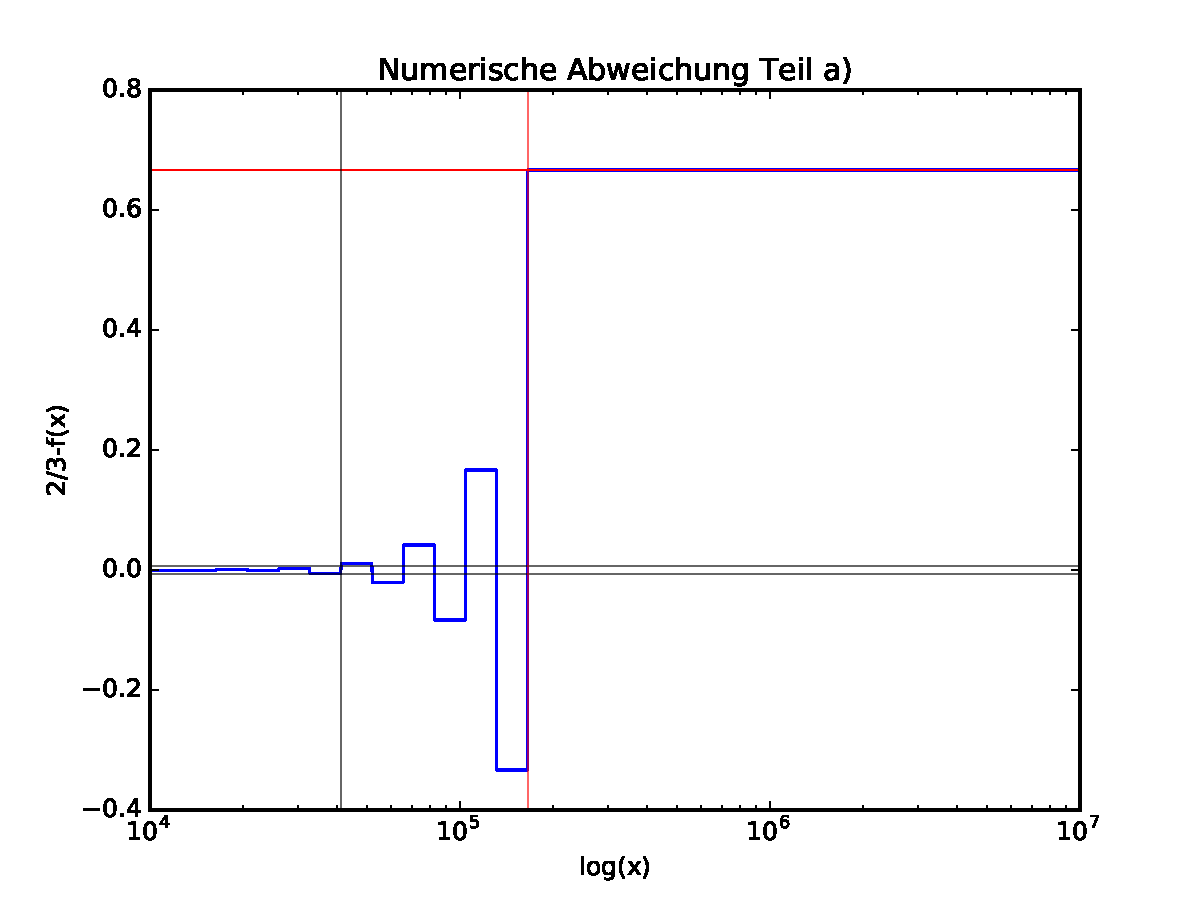
\includegraphics[width=0.6\textwidth]{plots/Aufgabe1a.pdf}
  \caption{Darstellung der Abweichung vom algebraischen Wert für die Funktion a).}
  \label{fig:A1a}
\end{figure}
\begin{figure}[H]
  \centering
  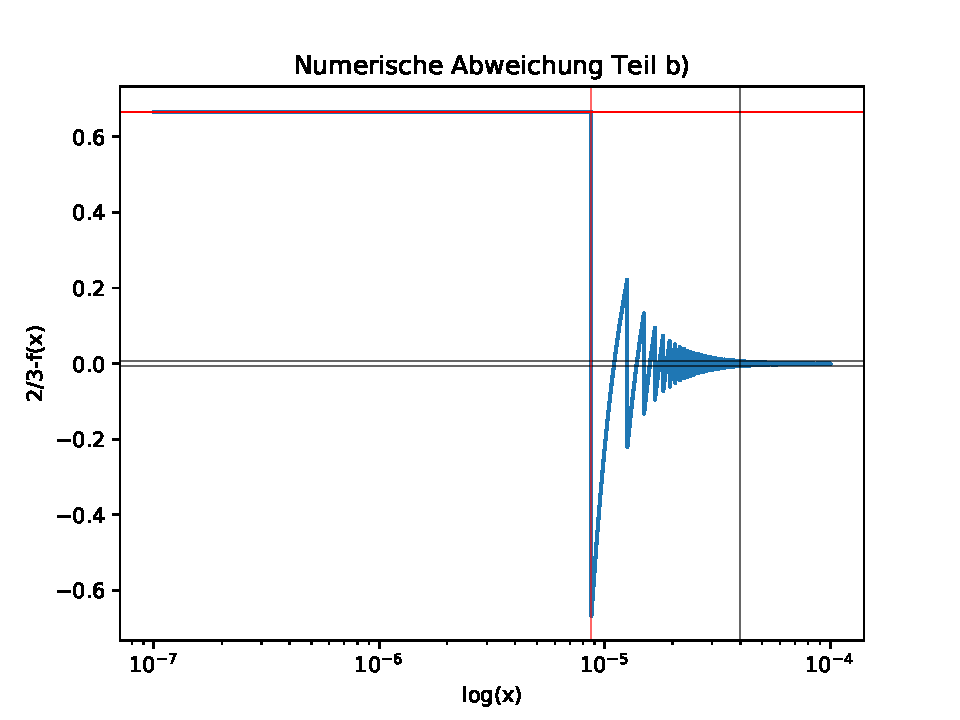
\includegraphics[width=0.6\textwidth]{plots/Aufgabe1b.pdf}
  \caption{Darstellung der Abweichung vom algebraischen Wert für die Funktion b).}
  \label{fig:A1b}
\end{figure}
